\section{Requirements}
\subsection{AI model}
% 사용자의 사진을 입력받아 뇌졸중의 여부를 판단하는 인공지능이다. 사람의 얼굴 사진으로 미리 학습을 시킨다. 이후 웹 서버에 배포를 해서 API를 통해 사진을 보내면 인식할 수 있다. 추론을 학습된 데이터를 기반으로 진행해 결괏값을 다시 API로 전송해 임의의 사람의 얼굴에 대한 뇌줄중 여부를 Face drooping을 근거로 판단하는 인공지능 모델이다.
This is an artificial intelligence system that takes user photos as input to determine the presence of a stroke. It is trained in advance with human facial photos. Subsequently, it is deployed on a web server, and by sending photos through an API, it can recognize whether there is a stroke. Inference is based on the trained data, and the results are sent back via an API, determining the presence of a stroke in an individual's face based on 'Face Drooping' as the criterion.\\

\subsection{Web communication}
% 웹 통신을 위해 다음과 같은 기능이 필요하다. AWS에 존재하는 인공지능 모델과 라즈베리 파이 사이의 통신을 지원한다. key, value로 이루어진 json 포맷으로 통신이 이루어지며 POST 방식으로 prdict가 이루어진다. 
For web communication, it is required that the system support communication between an artificial intelligence model existing on AWS and a Raspberry Pi. The communication takes place in json format, composed of key-value pairs, and predictions are made using the post method.\\
\subsubsection{Post}
% 웹으로 Post 할 때는 사용자의 이미지가 전달된다. 이미지가 Post 명령에 의해 전달되고 인공지능 모델이 인식할 수 있다. 인공지능 모델이 인식할 수 있도록 이미지를 변환하는 과정은 구현의 일관성을 유지하기 위해 아래의 handler에서 실행된다.
When posting on the web, the user's image is delivered. The image is delivered by post command and recognizable by the artificial intelligence model. The process of converting images so that artificial intelligence models can recognize them is executed in the handler below to maintain consistency in implementation.\\
\subsubsection{Get}
% 학습된 인공지능 모델이 Post된 자료를 받아 처리한 후 예측값을 다시 Raspberry Pi로 전해준다. 이 때, 값은 뇌졸중 가능성을 나타내는 확률값으로 정의된다. 단순히 0 또는 1로 판별하기에는 위험이 크다고 판단했기 때문이다.
The learned artificial intelligence model receives and processes the posted data and delivers the predicted value back to Raspberry Pi. In this case, the value is defined as a probability value indicating a stroke probability. This is because it was judged that there was a high risk to simply distinguish it as 0 or 1.\\

\subsection{AWS}

\begin{figure}[htp]
\centering

\includegraphics[width=4cm]{images/aws.png}
\caption{Amazon Web Service}
\label{fig:aws}
\end{figure}

% 인공지능 모델의 배포와 학습을 위한 서버이다. Ubuntu 기반의 x86-64로 구성되어 있다. EC2를 사용해 가상 인스턴스를 만들었으며 탄력적 IP로 접근 가능하도록 보안 설정을 했다.
It is a server for the deployment and training of the artificial intelligence model. It is built on an Ubuntu-based x86-64 architecture. We created a virtual instance using EC2 and configured security settings to make it accessible via an Elastic IP.\\

\subsection{Raspberry Pi}

\begin{figure}[htp]
\centering
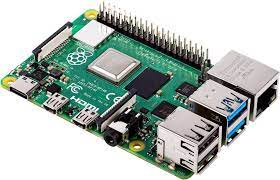
\includegraphics[width=4cm]{images/raspberrypi.jpeg}
\caption{Raspberry Pi}
\label{fig:raspberryPi}
\end{figure}

% 사용자의 사진을 촬영하는 카메라를 통제하고 촬영한 사진을 웹서버와 통신이 가능하게 한다. 인공지능 모델이 사진을 기반으로 뇌졸중 여부를 판단한 결과를 다시 받아 다시 사용자에게 알려주는 역할을 맡았다. 이 과정은 NUGU 스피커로 청각적으로나 Dashboard를 통해 시각적으로 표현이 가능하다.
It controls a camera that captures user photos and enables communication with a web server. The artificial intelligence model is responsible for determining the presence of a stroke based on the photos and relaying the results back to the user. This process can be conveyed either audibly through NUGU speakers or visually through a dashboard.\\

\subsection{Tensorflow Serving}

\begin{figure}[htp]
\centering

\includegraphics[width=4cm]{images/tensorflow.png}
\caption{TensorFlow}
\label{fig:tensorflow}
\end{figure}

% Tensorflow를 기반으로 인공지능 모델을 개발했을 때, 배포를 간편하게 진행할 때 필요하다.
When developing an artificial intelligence model based on TensorFlow, it is necessary for streamlined deployment.\\

\subsection{Handler}
% 학습된 인공지능 모델이 웹 서버에 존재할 때 전송되는 이미지 자료를 판단할 수 있도록 변형하고 전처리하는 과정과 예측한 결괏값을 API를 통해 돌려주기 위해 문자열을 제작하는 과정의 집합체이다. 이 기능을 통해 인공지능 모델의 배포와 유지관리를 쉽게 할 수 있다.
It is a collection of processes that involve transforming and preprocessing the image data sent to the web server to enable the trained artificial intelligence model to make assessments. It also involves generating strings to return the predicted results through an API. This functionality makes it easier to deploy and maintain the artificial intelligence model.\\

\subsection{Privacy Protection}
% 사용자의 사진을 촬영하는 카메라로서 사용되지 않는 경우에는 작동이 불가능해야 한다. 개인정보 보호를 위해 카메라가 작동 중이면 맥북의 웹캠처럼 표시를 가능하게 하거나 zoom의 기능과 같이 주변부를 흐리게 처리할 수 있다.
When not being used as a camera for capturing user photos, the camera should be non-operational. For privacy protection, if the camera is in operation, it should be capable of displaying a notification similar to the MacBook's webcam or applying a blur effect to the surroundings similar to the functionality in Zoom.\\

\subsection{NUGU}

\begin{figure}[htp]
\centering
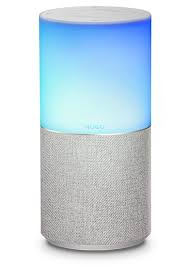
\includegraphics[width=3cm]{images/nugu.jpeg}
\caption{Nugu AI Speaker}
\label{fig:nugu}
\end{figure}

% 인공지능 스피커로 본 프로젝트에서는 라즈베리 파이에서 전송된 뇌졸중 여부를 사용자에게 청각적으로 전달할 수 있다. 이 외에 사용자가 원할 때 촬영을 시작하도록 trigger를 인식할 수 있다.
Using an artificial intelligence speaker gives the ability to audibly relay stroke information sent from the Raspberry Pi to the user. Additionally, the trigger could be used by the user to initiate photo capture when desired.\\

\subsection{Dashboard}
% 뇌졸중 여부를 시각적으로 표현해준다. 라즈베리 파이에서 전송된 뇌졸중 여부와 확률, chatGPT로 작성한 건강에 관련된 유용한 정보를 사용자에게 시각적으로 보여준다. 유용한 정보의 예시는 다음과 같다. 뇌졸중에 도움이 되는 음식이나 생활습관, 만약 발병한다면 어떻게 해야 하는지에 대한 정보가 포함된다.
It visually expresses whether you have a stroke or not. It displays stroke information and its probability sent from the Raspberry Pi, along with health-related useful information generated by ChatGPT, to the user. Examples of useful information include foods and lifestyle habits that can be beneficial in the event of a stroke, as well as guidance on what to do if a stroke occurs.\\
\subsubsection{Probability of Stroke}
% API를 통해 전송된 값에서 뇌졸중 여부의 확률값을 표현한다. 자동차의 속도 계기판을 모티브로 하여 사용자에게 직관적으로 확률을 전달한다.
It expresses the probability value of stroke from the value transmitted through the API. It transmits probabilities to users by using as a motif the speed dashboard of a car.\\
\subsubsection{User's Image}
% 사용자를 촬영한 사진을 보여준다. 이로써 사용자는 자신의 상태를 객관적으로 확인할 수 있으며 경각심을 일으킬 수 있다.
It displays the photo of the user, allowing the user to objectively assess their own condition and potentially raise awareness of their health.\\
\subsubsection{Treatment Options}
% 아래의 chatGPT를 통해 얻은 뇌졸중의 치료법을 보여주는 공간이다. 만약 사용자가 뇌졸중의 확률이 높을 경우에는 더욱 눈에 띄도록 표현할 수 있다.
It shows treatment options obtained using ChatGPT. If the user has a high probability of stroke, these treatment options can be highlighted in order to draw even more attention to the user.\\
\subsubsection{Prevention and Information}
% 아래의 chatGPT를 통해 얻은 뇌졸중의 예방법을 알려준다. 뇌졸중의 확률이 낮더라도 예방법을 사용자에게 알려주고, 만약 의심될 때는 어떻게 해야하는지 행동지침을 알린다. 이로써 능동적인 건강관리를 가능케 한다. 
It tells users how to prevent themselves of gettting a stroke obtained and this information is also obtained by using ChatGPT. Even if the probability of stroke is low, it still informs the user of preventions and informs him on the behavioral guidelines to have in suspicion of stroke. This enables daily active health care.\\

\subsection{ChatGPT}

\begin{figure}[htp]
\centering

\includegraphics[width=2.5cm]{images/chatgpt.png}
\caption{ChatGPT}
\label{fig:chatgpt}
\end{figure}

% 사용자의 뇌졸중 여부와 확률을 기반으로 유용한 정보를 생성해주는 생성형 AI이다. API를 이용해서 질문을 담아서 전송하고 답변을 다시 받아온다. 그 답변을 Dashboard 혹은 NUGU를 통해 사용자에게 알려준다. 
It is a generative AI that generates useful information based on the user's stroke status and probability. It uses API to send questions and receive answers. The answer is notified to the user through the Dashboard or the NUGU Speaker.\\
\subsubsection{Question}
% chatGPT에게 뇌졸중 관련으로 질문할 때 피상적인 표현으로 한다면 당장 병원에 가야한다는 정보만 얻는다. 인공지능 모델이 반환한 결괏값에서 확률을 추출하고 치료법과 예방법, 병원을 어떻게 골라야하는지를 직접적으로 물어본다. 
When asking questions related to strokes to ChatGPT, you only receive information suggesting an immediate need to go to the hospital. By extracting the probability from the results returned by the artificial intelligence model, we can inquire directly about treatment options, preventive measures, and guidance on selecting a hospital.\\
\subsubsection{Answer}
% 위의 질문 형식으로 chatGPT에게 질문하고 받은 대답이다. 이 대답은 Dashboard 혹은 NUGU로 전달되어 각각 시각적, 청각적인 표현으로 사용자에게 전달된다.
After using the question format above, the answer received from ChatGPT can be passed to the Dashboard or the NUGU Speaker then passed to the user in a visual or auditory representation.\\

\subsection{Database}
% 인공지능 모델의 정확도를 향상시키기 위해서 이미지를 보관하는 데이터베이스가 필요할 수 있다. 하지만 이는 개인정보로 민감할 수 있기에 데이터베이스 없이 프로젝트를 구현하는 것으로 진행할 수도 있다.
To enhance the accuracy of the artificial intelligence model, a database for storing images may be required. However, since this can involve sensitive personal information, the project can also be implemented without a database.\\